\chapter*{Introduction}
\label{cap:introduction}
\addcontentsline{toc}{chapter}{Introduction}

In recent yars, the advancement of immersive technologies such as \gls{vr} has brought about a significant change in how users interact in digital environments.
Major companies like Meta and Apple have invested in the development of hardware for these technologies, launching devices like the Meta Quest 3 and Apple Vision Pro, and creating social interaction platforms in the \gls{metaverse} with the development of Meta Horizon Worlds.
This technology has opened new opportunities to explore more natural modes of communication in virtual spaces through non-verbal communication.

Non-verbal communication refers to the transmission of messages without the use of words, relying instead on images and gestures.
In our daily lives, it plays a crucial role in human interactions, yet its representation in virtual environments is often limited and dependent on predefined actions such as animations or "emotes" already integrated into the game.
Therefore, the development of tools that can capture and interpret these gestures in real-time represents a significant step towards creating more expressive and realistic virtual environments.
\section{Motivation}


As mentioned in the introduction, the use of non-verbal communication in virtual environments is limited and predefined by their design, restricting a fundamental part of everyday human expression.
Due to this, and as seen in articles like \cite{Neverova} or \cite{VRHANDS}, gesture detection is a field of study currently being explored to address this issue.
For these reasons, it is interesting to investigate ways to expand this representation of non-verbal communication so that interaction between users and \glspl{npc} becomes more natural.

This work is therefore part of the research line focused on developing tools that can recognize gestures performed by a user using a motion capture suit, with the aim of creating more immersive and natural virtual environments for users.
On the other hand, a large amount of data is required to create \gls{ai} models that enable the development of the mentioned tools.
In the case of this project, the necessary data consists of a sequence of 3D coordinates representing the positions and rotations of the skeleton's bones throughout the animations, resulting in relatively large data sizes.
This necessitates the creation of complex models capable of processing a significant amount of input data. However, as we will discuss throughout the work, it has not been possible to find datasets containing this type of data.
As a result, a significant contribution of this work to the field has been the creation of a dataset through the extraction of animations from a specialized bank and the motion capture of users.

Given these reasons, it can be concluded that the lack of natural methods to leverage non-verbal communication in virtual environments and the scarcity of animation datasets have motivated the objectives mentioned, which we will expand upon below.

\section{Objectives}

The general objective of this project is to implement an \gls{ai} model that, with low latency, allows real-time identification of gestures performed with a motion capture suit, aiming to enhance non-verbal communication in virtual environments.
To achieve this objective, the following goals have been proposed during the development of the work:
\begin{enumerate}
	%\renewcommand{\theenumi}{\alph{enumi}}
	\item Search for animation datasets that are considered relevant for communicating with an \gls{npc} in a video game. These animations include dancing, greeting, pointing, sitting, fighting, and running.
	\item Automatic extraction of the aforementioned animations from animation banks and subsequent processing.
	\item Extraction of animations through motion capture from a heterogeneous group of users.
	\item Implementation, training, and comparison of different \gls{ai} models, including neural networks (LSTM, CNN, and RNN) as well as classical classification models (Random Forest).
	\item Development of a final application as a demonstration to showcase the results in \gls{vr} to enhance immersion.
\end{enumerate}

As a significant secondary objective, due to the lack of animation datasets, it has been proposed to publish the resulting datasets, both from artificial animations and user captures.

\section{Work Plan}


The work plan consists of several steps:

\begin{enumerate}
	%\renewcommand{\theenumi}{\alph{enumi}}
	\item Search for a dataset: generate a sufficiently large dataset with multiple examples of gestures to adequately train different models. This dataset should primarily consist of data from real users to identify the most natural gestures possible.
	\item Implementation of \gls{ai} models: implement various \gls{ai} models to compare them and determine which one is most suitable based on prediction speed and accuracy. The implementation of these models should include: training, a way to extract final model statistics, hyperparameter search, confusion matrix generator, and compatibility with a common user interface for all trainings.
	\item Development of a user interface for training and monitoring different models: develop a web interface so that users with less programming and \gls{ai} experience can train models capable of predicting the gestures they need without modifying the code or needing to understand the internal workings of the codebase.
	\item Development of a final application: create an application for Oculus Quest as a demo that connects to the chosen model and allows real-time usage demonstration.
\end{enumerate}

The development of tasks and their planning can be seen in Figure \ref{fig:diagrama-gantt-eng}.

\begin{figure}[H]
	\centering
	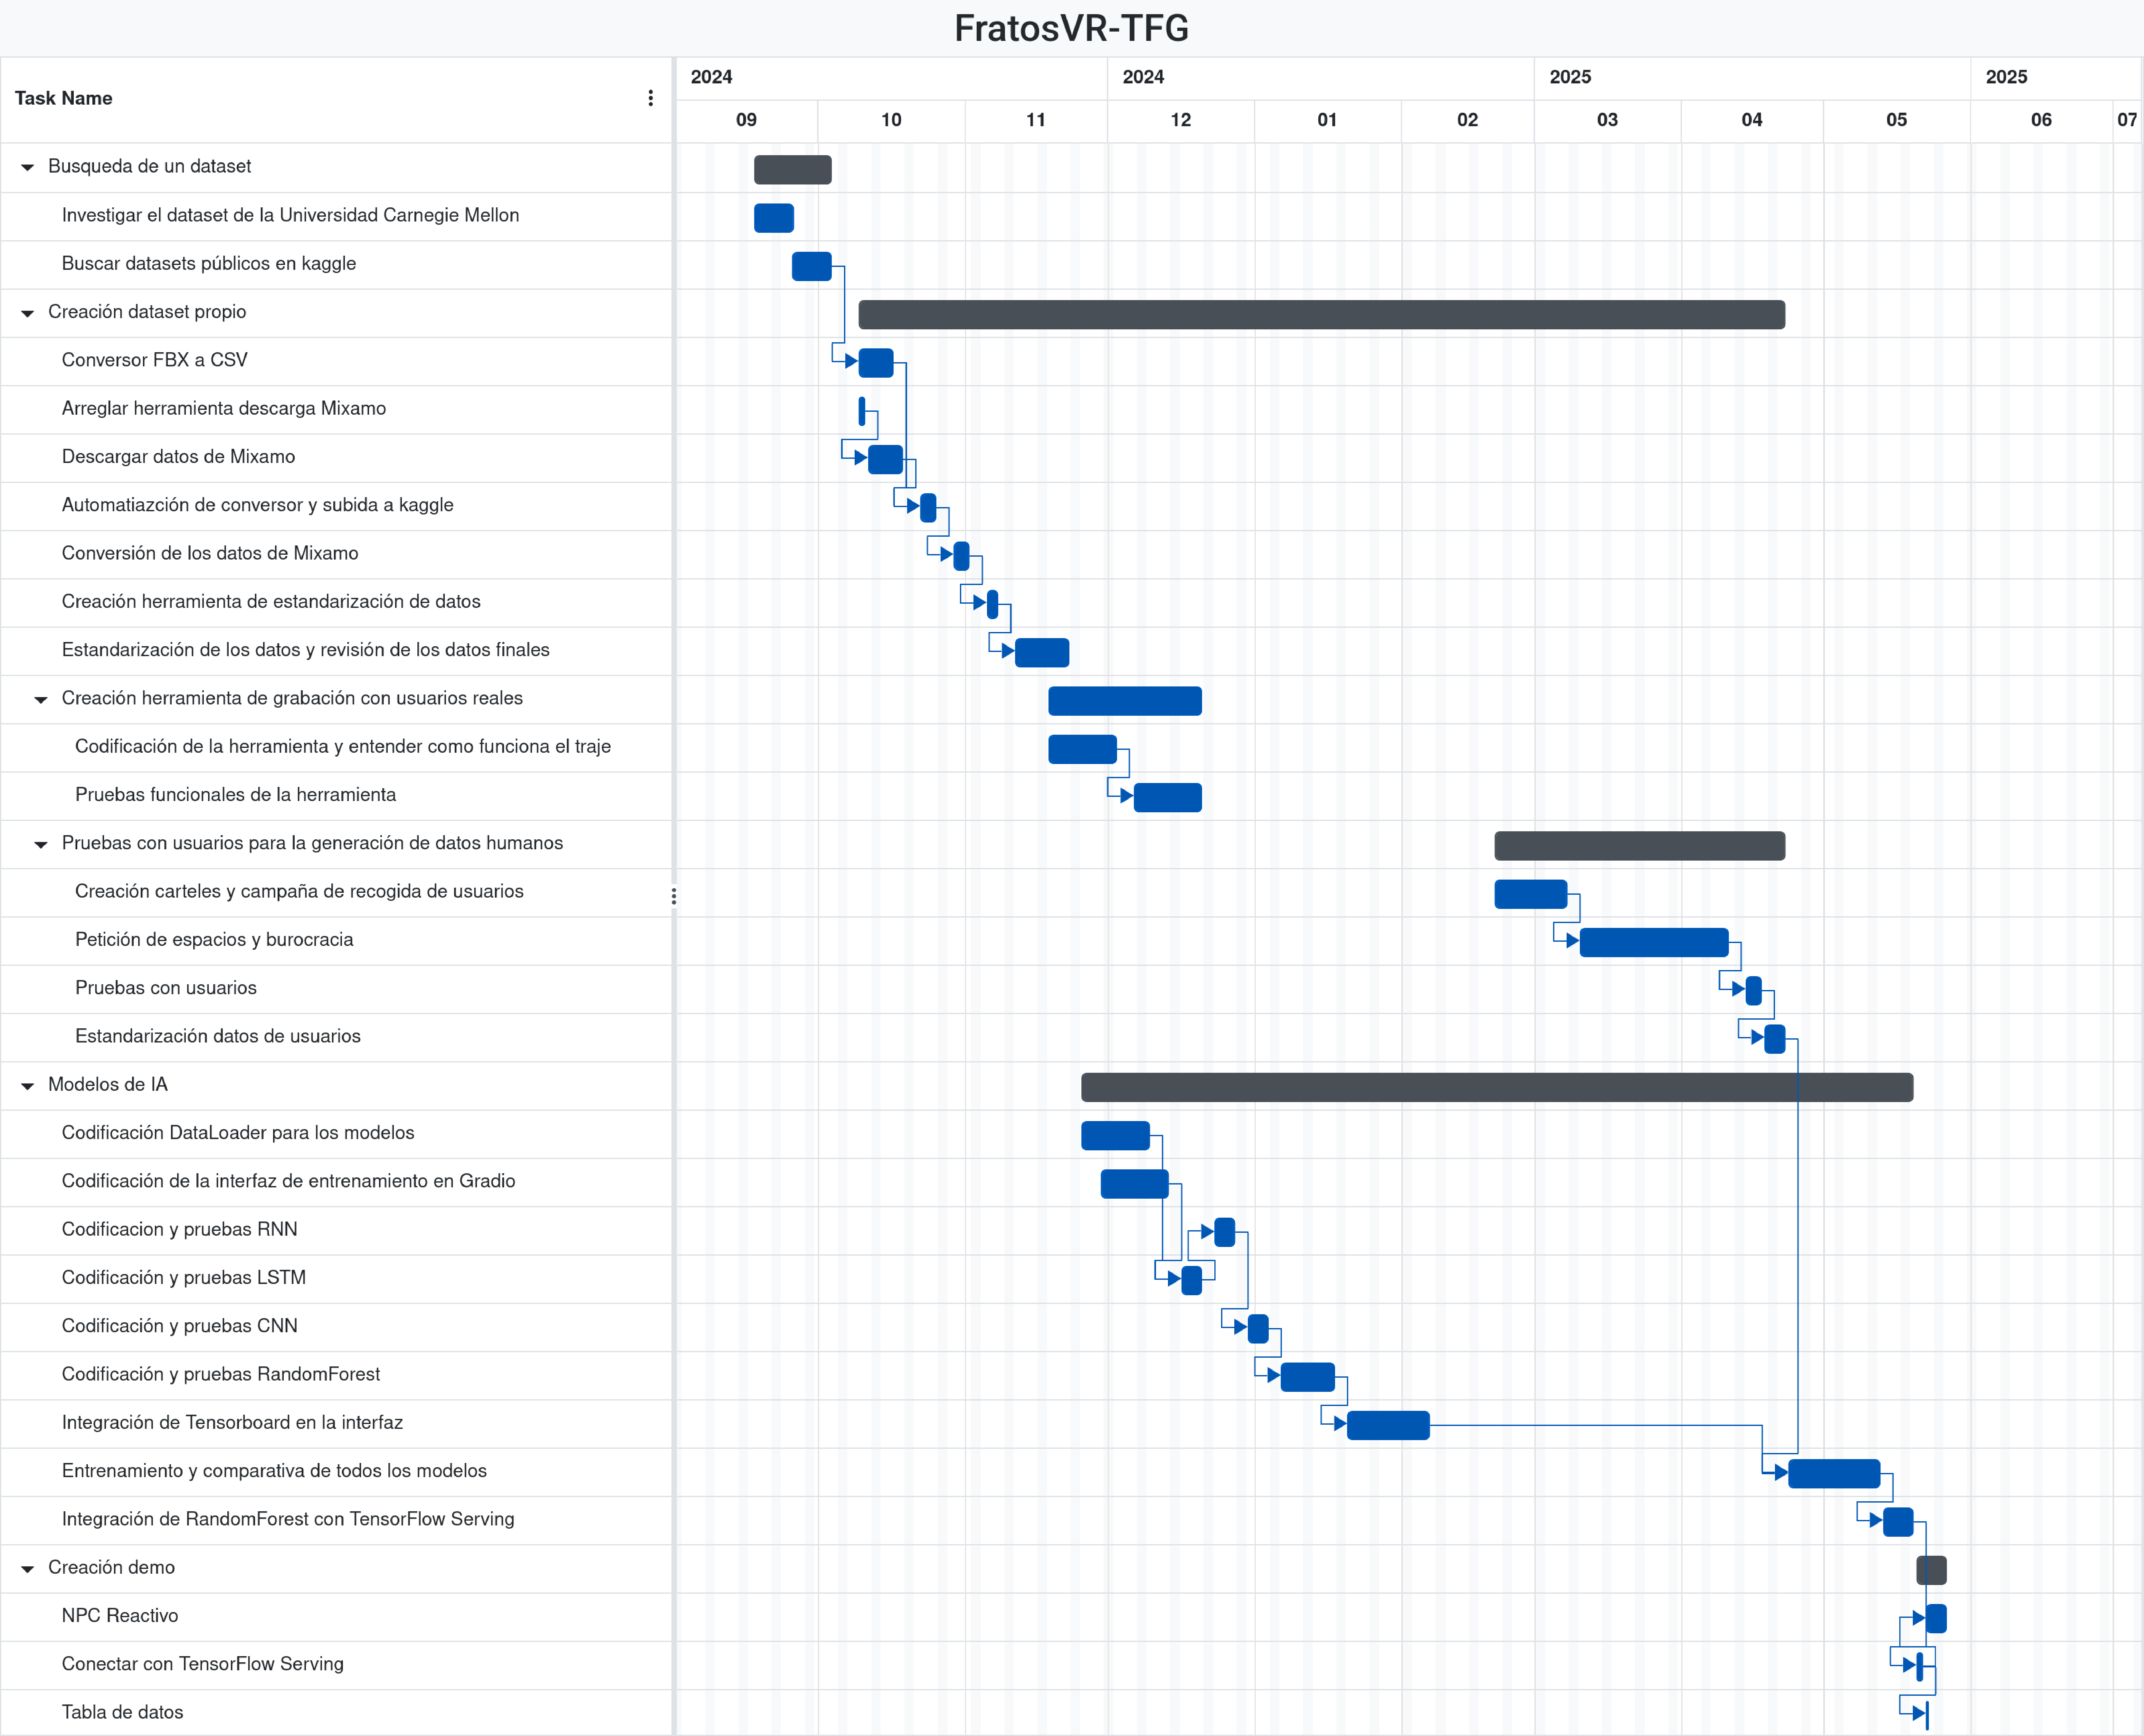
\includegraphics[width=0.91\textwidth]{Imagenes/Vectorial/Diagrama-gannt.pdf}
	\caption{Gantt chart of the project}
	\label{fig:diagrama-gantt-eng}
\end{figure}